
\chapter{Управляемая динамика квадрокоптера с поворотными роторами}

\section{Основные элементы конструкции квадрокоптера с поворотными роторами}

Основным элементом конструкции БЛА является корпус, из которого выходят лучи с закрепленными на концах двигателями с пропеллерами. Лучи расположены симметрично относительно корпуса аппарата и реализуют так называемую Х-схему. Смежные пропеллеры имеют противоположное направление вращения; первый и третий – пропеллеры левого вращения, а второй и четвертый – правого. Каждый из роторов может поворачиваться посредством сервопривода вокруг продольной оси луча, на котором он закреплен. Для построения математической модели динамики БЛА условимся, что он сконструирован таким образом, что
\begin{itemize}
	\item главные центральные оси инерции аппарата и каждого из роторов совпадают с осями симметрии; 
	\item корпус БЛА и каждый из четырех роторов являются твердыми телами; 
	\item под ротором будем понимать вращающуюся часть двигателя и пропеллер, которые являются одним телом; 
	\item крепление роторов к корпусу БЛА происходит в точке, совпадающей с центрами масс роторов, помимо роторов спрпелеерами в системе отсутствуют подвижные части;
	\item центры масс роторов лежат на окружности радиуса $L$, центр окружности совпадает с центром масс корпуса аппарата.
\end{itemize}
Общий вид аппарата представлен рисунке \ref{fig:tiltrotor_scheme}.

\section{Постановка задачи управления}
\label{section_ctrl_task}

Считая заданной требуемую траекторию БЛА в координатном пространстве, положим целью управления обеспечение наперёд заданной траектории центра масс аппарата, а также требуемой ориентации. Такая постановка позволяет формализовать следующие задачи:
\begin{itemize}
\item приведение центра масс БЛА в некоторое наперёд заданное статичное положение;
\item стабилизация ориентации БЛА относительно некоторого наперёд заданного положения;
\item перемещение центра масс БЛА вдоль некоторой наперёд заданной (дискретным набором точек или как непрерывная функция координат от времени) траектории;
\item слежение за объектом, перемещающимся произвольным образом;
\item наведение камеры, установленной на БЛА на неподвижный или перемещающийся объект (то есть съёмка неподвижного объекта с разных ракурсов или слежение камерой за подвижным объектом).
\end{itemize}

Решение последней задачи в явном виде использует степени свободы, связанные с увеличением размерности вектора управляющих параметров. Стоит отметить, что квадрокоптер со стандартной конструкцией произвольный манёвр наведения камеры в точку с одновременным изменением высоты выполнить не способен.
\begin{figure}[h]
	\centering
	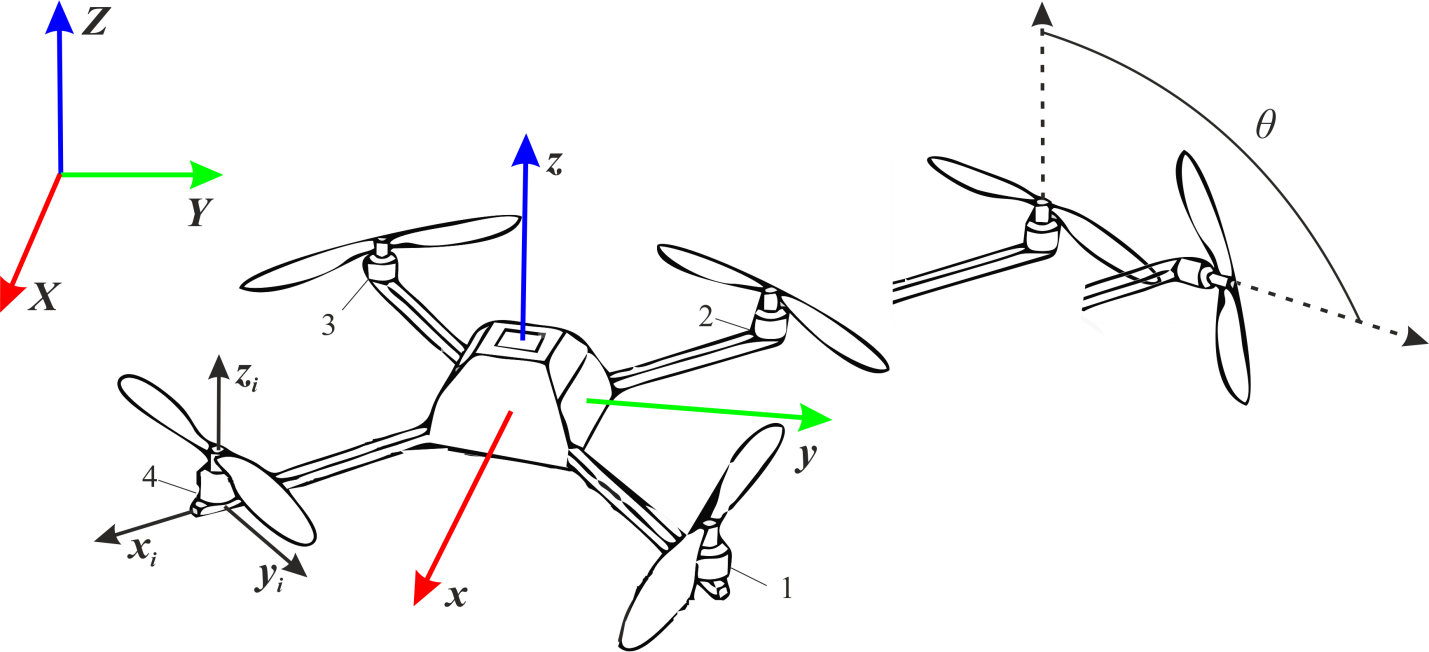
\includegraphics[scale=0.9]{tiltrotor_scheme}
	\caption{ -- Общая схема квадрокоптера с поворотными роторами}
	\label{fig:tiltrotor_scheme}
\end{figure}

\section{Математическая модель динамики БЛА}

Движение аппарата рассматривается относительно неподвижной инерциальной системы отсчета $I$, связанной с Землей (вращением Земли на характерных временах автономного полёта БЛА рассматриваемого класса принято пренебрегать).
Направление осей выбрано по схеме «Восток, Север, Верх» (ENU) -- ось \textbf{$X_I$} направлена на восток, ось \textbf{$Y_I$} -- на север, а ось \textbf{$Z_I$} -- от центра Земли.

Индексом $B$ обозначим жестко связанную с корпусом аппарата систему координат с началом в центре масс и осями, совпадающими с главными центральными осями инерции корпуса БЛА.
Для промежуточных выкладок нами будет использована ещё одна жестко связанная с корпусом система координат $B'$, полученная из $B$ поворотом вокруг оси $Z_B$ таким образом, что ось $X_B'$ направлена вдоль луча, несущего первый ротор согласно схеме \ref{fig:tiltrotor_scheme}.

Индексами $R_i$ будем обозначать системы координат, жестко связанные с роторами и совпадающие с их главными центральными осями инерции.

При записи векторов будем отмечать верхним индексом систему координат, в которой записано разложение вектора. Повороты систем координат друг относительно друга будем описывать кватернионами. Будем говорить, что кватернион $q_{IB}$ задаёт ориентацию системы координат $B$ относительно $I$ в том смысле, что разложения некоторого вектора $\bm{r}$ в этих двух базисах связаны соотношением
\begin{equation} \label{eq:m_quat}
\bm{r}^I = q_{IB} \circ \bm{r}^B \circ \tilde{q}_{IB}.
\end{equation}

Положение БЛА в пространстве определяется радиус-вектором его центра масс $\bm{r}^I$ и кватернионом ориентации $q_{IB}$. Скорость центра масс аппарата равна
\begin{equation} \label{eq:m_vel}
\bm{v}^I = \dot{\bm{r}^I}.
\end{equation}
Изменение кватерниона ориентации аппарата определяется уравнением Пуассона
\begin{equation} \label{eq:m_puasson}
\dot{q}_{IB} = \frac{1}{2} {q}_{IB} \circ \bm{\Omega}^B,
\end{equation}
где $\bm{\Omega}_B$ – угловая скорость корпуса БЛА в проекции на собственные оси.

Движение центра масс БЛА определяется уравнением
\begin{equation} \label{eq:m_traslational_motion}
\ddot{\bm{r}} = M \bm{g}^I - \frac{1}{2} \rho C S_{\perp} |\bm{v}^I| \bm{v}^I + \sum_{i=1}^{4}{ { (-1)^{i+1} k \tilde \omega_i |\tilde \omega_i| \bm{e}^I_{z_i}}},
\end{equation}
где три члена в правой части соответствуют силе тяжести, силе аэродинамического сопротивления и создаваемой пропеллерами тяге, $M = m + \sum_{i=1}^{4}{m_i}$ – общая масса корпуса, $m_i$ – масса $i$-го ротора с пропеллером, $\bm g$ – ускорение свободного падения, $S_{\perp}$ – площадь миделева сечения корпуса аппарата, $C$ – аэродинамический коэффициент сопротивления воздуха, $\bm{e}^I_{z_i}$ – единичный вектор вдоль оси симметрии i-го ротора, $k$ – аэродинамический коэффициент, определяемый экспериментально; $\tilde \omega_i$ – скорость вращения i-го пропеллера.

Для описания вращательного движения воспользуемся динамическими уравнениям Эйлера
\begin{equation} \label{eq:m_rotational_motion}
\bm{\tau}^{B} =
\bm{J}_B\dot{\bm{\Omega}}^B + \bm{\Omega}^B \times \bm{J}_B{\bm{\Omega}^B},
\end{equation}
где $\bm{J}_B$ — тензор инерции корпуса в главных осях корпуса; $\bm{\tau}^{B}$ —
главный момент сил, действующий на корпус.

Главный момент сил складывается из моментов сил, действующих на корпус аппарата со стороны поворотных роторов с пропеллерами и внешних моментов:
\begin{equation} \label{eq:m_general_torq}
\bm{\tau}^{B} =
-\sum_{i=1}^{4} {\bm{\tau}^{B}_i} +
\sum_{i=1}^{4} {\bm{r}^B_i \times (-1)^{i+1} k \tilde \omega_i |\tilde \omega_i| \bm{e}^I_{z_i},}
\end{equation}
где $\bm{\tau}^{B}_i$ — моменты сил, действующие на роторы со стороны аппарата, $\bm{r}^B_i$ -- радиус вектор, проведенный из центра масс квадрокоптера $i$-тому к ротору. Вычислим угловую скорость $i$-го ротора в проекциях на оси $R_i$:
\begin{equation} \label{eq:m_prop_ang_vel}
\bm{\omega}^{R_i}_i =
q_{{R_i} B} \circ (\bm{\Omega}^B + \dot {\theta}_i \bm e^B_{r_i}) \circ \tilde {q}_{{R_i}B} +
\tilde \omega_i \bm{e}^{R_i}_{z_i},
\end{equation}
где $\bm e^B_{r_i}$ -- орт вектора $\bm{r}^B_i$, ${\theta}_i$ -- угол поворота $i$-того ротора. Запишем динамические уравнения Эйлера для ротров.
\begin{equation} \label{eq:m_rotors_dyn}
\bm{\tau}^{{R_i}}_i + \bm{\varsigma}^{{R_i}}_{i} = 
\bm{J}_{R_i}\dot{\bm{\omega}}^{R_i}_i + \bm{\omega}^{R_i}_i \times \bm{J}_{R_i}{\bm{\omega}^{R_i}_i},
\end{equation}
где $\bm{J}_{R_i}$ -- тензор инерции $i$-того ротора с пропеллером, записанный в собственных главных осях, $\bm{\varsigma}^{{R_i}}_{i}$ -- внешний момент силы, для которго запишем:
\begin{equation} \label{eq:m_ext_torq}
\begin{aligned}
&\bm{\varsigma}^{{R_i}}_{i} = -b \tilde \omega_i |\tilde \omega_i| \bm e^{R_i}_{r_i}\\
&\bm{\varsigma}^{B}_{i} = q_{ B {R_i}} \circ \bm{\varsigma}^{{R_i}}_{i} \circ \tilde q_{ B {R_i}}.
\end{aligned}
\end{equation}
Здесь $b$ -- аэродинамический коэффициент, определяемый экспериментально.

Окончательно уравнения вращательной динамики аппарата принимают вид:
\begin{equation} \label{eq:m_final_rotational_motion}
\begin{aligned}
\bm{J}_B\dot{\bm{\Omega}}^B + \bm{\Omega}^B \times \bm{J}_B{\bm{\Omega}^B} =
&\sum_{i=1}^{4} {\bm{r}^B_i \times
	(-1)^{i+1} k \tilde \omega_i |\tilde \omega_i| \bm{e}^I_{z_i}} + \\ +
\sum_{i=1}^{4} {\bm{\varsigma}^{{R_i}}_{i}} +
&\sum_{i=1}^{4} q_{ B {R_i}} \circ (\bm{J}_{R_i}\dot{\bm{\omega}}^{R_i}_i + \bm{\omega}^{R_i}_i \times \bm{J}_{R_i}{\bm{\omega}^{R_i}_i}) \circ \tilde q_{ B {R_i}}
\end{aligned}
\end{equation}
Уравнения (\ref{eq:m_vel}), (\ref{eq:m_puasson}), (\ref{eq:m_traslational_motion}) и (\ref{eq:m_final_rotational_motion}) составляют замкнутую систему, позволяющую моделировать динамику полета квадрокоптера с поворотными роторами.

\section{Синтез регулятора}

Пусть задана требуемая траектория центра масс аппарата $\bm r^0(t)$, а также требуемая ориентация $q^0(t)$. Обозначим  $\delta \bm r(t) = \bm r^0(t) - \bm r(t)$ и $\delta q(t) = q^0(t) \circ \tilde q(t)$, где $\delta \bm r$ и $\delta q$ определяют расхождение требуемой и текущей траектории БЛА в координатном пространстве, а $q = q_{IB}$.  В качестве переменных управления выберем скорости вращения пропеллеров ${\tilde \omega}_i$ и углы поворота роторов ${\theta}_i$:
\begin{equation} \label{eq:m_ctrl_out}
\begin{aligned}
	&\bm{u} = (\bm \omega_u, \bm \theta_u)^T,
	\\
	\bm \omega_u =
	(\tilde\omega_1 |\tilde\omega_1|,
	\tilde\omega_2 |\tilde\omega_2|&,
	\tilde\omega_3 |\tilde\omega_3|,
	\tilde\omega_4 |\tilde\omega_4|)^T,
	\quad
	\bm \theta_u = (\theta_1, \theta_2 , \theta_3 , \theta_4 )^T.
\end{aligned}
\end{equation}
Регуляторы, обеспечивающие необходимое управление по положению и ориентации могут быть построены, как
\begin{equation} \label{eq:m_reg}
\begin{aligned}
	\ddot{\bm{r}_d}(t)&=
	\ddot{\bm{r}}^0(t)+\bm{K}_{r1}(\dot{\bm{r}}^0(t) - \dot{\bm{r}}(t))+\bm{K}_{r2}\delta \bm r,\\
	\dot{\bm{\Omega}}_d(t)&=
	\dot{\bm{\Omega}}^0(t)+\bm{K}_{\Omega1}(\bm{\Omega}^0(t)-\bm{\Omega}(t))+\bm{K}_{\Omega2}\delta\bm{q},
\end{aligned}
\end{equation}
где $\delta \bm q$ -- векторная часть кватерниона $\delta q$,
$\ddot{\bm{r}}^0$, $\dot{\bm{r}}^0$, $\ddot{\bm{\Omega}}^0$, $\dot{\bm{\Omega}}^0$ -- целевое ускорение, скорость, угловое ускорение и угловая скорость соответственно,
$\bm K_{r1}$, $\bm K_{r2}$, $\bm K_{\Omega1}$, $\bm K_{\Omega2}$ -- диагональные матрицы коэффициентов, выбор которых согласно критерию Рауса-Гурвица гарантирует сходимость траектории аппарата к требуемой. Таким образом, для построения
контура управления, необходимо связать выход из регулятора с управляющими
параметрами, учесть присутствующие в системе ограничения на реализацию
управляющих воздействий, а также реализовать обратные связи.

\section{Обращение динамики модели}
\label{section_dyn_inverse}

Реализация контура управления с регуляторами (\ref{eq:m_reg}) требует обращения динамики системы, то есть определения значений всех управляющих параметров (\ref{eq:m_ctrl_out}) по выходу из регулятора (\ref{eq:m_reg}).
Для достижения этой цели преобразуем уравнения модели (\ref{eq:m_vel}), (\ref{eq:m_puasson}), (\ref{eq:m_traslational_motion}), (\ref{eq:m_final_rotational_motion}).
Сначала перепишем их в проекциях на оси системы координат $B'$, а затем
преобразуем таким образом, чтобы в правой части получившихся выражений остались все члены, в которые явно входят управляющие параметры (\ref{eq:m_ctrl_out}), а все остальные члены перенесём в левую часть. Таким образом, получим систему уравнений
\begin{equation} \label{eq:m_dyn}
\begin{aligned}
&\bm F(\ddot{\bm r}_d, \dot{\bm r}, q) = k F_{thr} (\bm \theta_u) \bm \omega_u,\\
&\bm T(\dot{\bm \Omega}_d, \bm\Omega) = \Big(
kLT_{thr}(\bm\theta_u) - bT_{aero}(\bm\theta_u)
\Big)
\bm \omega_u.
\end{aligned}
\end{equation}

Система (\ref{eq:m_dyn}) недоопределена и нелинейна относительно компонент $\bm \theta_u$, что значительно затрудняет ее аналитическое решение. Доопределим систему, используя выражения для распределения вертикальных составляющих сил и моментов между парами двигателей, расположенных на параллельных лучах
\begin{equation} \label{eq:m_dyn_balance_1}
\begin{aligned}
&k \tilde\omega_1 |\tilde\omega_1| c_1 + k \tilde\omega_3 |\tilde\omega_3| c_3 =
\frac{1}{2} \bm F_z + \epsilon_F,
\\
&\tilde\omega_1 |\tilde\omega_1| (bc_1 - kLs_1)
+ \tilde\omega_3 |\tilde\omega_3| (bc_3 - kLs_3) =
\frac{1}{2} \bm T_z + \epsilon_T,
\end{aligned}
\end{equation}

\begin{equation} \label{eq:m_dyn_balance_2}
\begin{aligned}
&k \tilde\omega_2 |\tilde\omega_2| c_2 + k \tilde\omega_4 |\tilde\omega_4| c_4 =
-\frac{1}{2} \bm F_z + \epsilon_F,
\\
&\tilde\omega_2 |\tilde\omega_2| (bc_2 + kLs_2)
+ \tilde\omega_4 |\tilde\omega_4| (bc_4 + kLs_4) =
\frac{1}{2} \bm T_z - \epsilon_T,
\end{aligned}
\end{equation}
где $\epsilon_F$ и $\epsilon_F$ -- балансировочные параметры.

Полученная система уравнений (\ref{eq:m_dyn}), (\ref{eq:m_dyn_balance_1}) имеет аналитическое решение:
\begin{equation} \label{eq:m_dyn_resolve}
\begin{aligned}
&\tilde\omega_i |\tilde\omega_i| =
\frac{(-1)^{i+1}}{2kL}\Big(
A^2_i + 
B^2_i
\Big)^{\frac{1}{2}},
\\
\phantom{}
\\
&\theta_i = 
2 \arctan \Bigg[(-1)^{i+1}	
\frac{A_i -
\Big(A^2_i +
B^2_i
\Big)^{\frac{1}{2}}}
{B_i}
\Bigg],
\end{aligned}
\end{equation}
где $A_i = A_i(\bm F, \bm T, \epsilon_F, \epsilon_T)$
и
$B_i = B_i(\bm F, \bm T, \epsilon_F, \epsilon_T)$
-- скалярные функции, куда линейно входят компоненты левой части уравнений динамики \eqref{eq:m_dyn}
$\bm F(\ddot{\bm r}_d, \dot{\bm r}, q)$
и
$\bm T(\dot{\bm \Omega}_d, \bm\Omega)$.
Таким образом, полученное решение связывает выход регулятора с управляющими параметрами при наличии обратной связи, а именно известных текущих координате $\bm r^I$, скорости $\bm v^I$, ориентации $q_{IB}$ и угловой скорости $\bm \Omega^B$.


\section{Введение ограничений на компоненты вектора управляющих воздействий}
\label{section:limits}

Ограничим максимальные значения оборотов двигателей и угды отклонения сервоприводов некоторыми значениями:
\begin{equation} \label{eq:m_limits_init}
\begin{aligned}
&0< (-1)^{i+1} \tilde \omega_i |\tilde\omega_i| < \tilde \omega_{max}^2,
\\
&|\theta_i| < \theta_{max} < \pi.
\end{aligned}
\end{equation}

Используя уравнения обращенной динамики (\ref{eq:m_dyn_resolve}), можно переписать ограничения (\ref{eq:m_limits_init}) в виде
\begin{equation} \label{eq:m_limits_AB}
\begin{aligned}
&0 <
\sqrt{A^2_i +  B^2_i}
< 2 k^2 L\omega_{max}^2,
\\
&\Bigg|\frac{A_i-\sqrt{A^2_i +  B^2_i}}{B_i}\Bigg| < 
\tan\frac{\theta_{max}}{2}.
\end{aligned}
\end{equation}
Найдем область в пространстве $(A_i, B_i)$, в которой будут выполнены данные ограничения. Выполним замену переменных
\begin{equation} \label{eq:m_polar}
\begin{aligned}
&A_i = \rho_i \cos(\phi_i),
\\
&B_i = \rho_i \sin(\phi_i).
\end{aligned}
\end{equation}
Тогда выражения (\ref{eq:m_limits_AB}) примут вид
\begin{equation} \label{eq:m_limits_polar_rho}
0 < \rho < 
2 k^2 L\omega_{max}^2
= \rho_{max},
\end{equation}
\begin{equation} \label{eq:m_limits_polar_phi}
\Bigg| \frac{\cos(\phi_i)-1}{\sin(\phi_i)} \Bigg| < 
tg\frac{\theta_{max}}{2}.
\end{equation}
Преобразовав
(\ref{eq:m_limits_polar_rho}),
(\ref{eq:m_limits_polar_phi}),
получим:
\begin{equation} \label{eq:m_limits_new_1}
\sqrt{A^2_i +  B^2_i} <
\rho_{max}
\end{equation}
\begin{equation} \label{eq:m_limits_new_2}
|B_i| < A_i \tan \theta_{max}
\end{equation}

Условия \eqref{eq:m_limits_new_1}, \eqref{eq:m_limits_new_2} формируют область $\Omega_{A_iB_i}$ на плоскости $A_iB_i$, в которой выполняются необходимые ограничения на выходы управления. Область является внутренними точками сектора круга радиуса $\rho_{max}$ и центральным углом $2\theta_{max}.$ Можно показать, что данная область эквивалентна некоторой области $\Omega_{\bm{y}}$ в пространстве вектора  $\bm{y} \in \mathcal{R}^6$, $\bm{y} = (\bm{F}, \bm{T})^T$, из которой можно выделить прямоугольную область $\Psi_{\bm y} \in \Omega^*_{\bm y}$, тем самым независимо определить ограничения на каждый из компонент вектора $\bm y$
\begin{equation} \label{rect_in}
y_k^{min} < y_k < y_k^{max},
\quad k = 1 .. 6.
\end{equation}

Таким образом, ограничив выходы регулятора таким образом, чтобы выполнялись соотношения \eqref{eq:m_limits_new_1}, \eqref{eq:m_limits_new_2}, мы гарантируем выполенение необходимых ограничений \eqref{eq:m_limits_init} на компоненты вектора управляющих воздействий.

\section{Экстренное управление при отказе двух смежных двигателей}
\label{section_em_ctrl}

Как было показано в этой главе, расширение размерности вектора управляющего воздействия квадрокоптера позволяет повысить маневренные характеристики аппарата и помогает добиться независимого управления по всем 6-ти степеням свободы.
Однако, при возникникновении нештатной ситуации способность изменять вектор тяги каждого из двигателей может спасти аппарат от неконтролируемого падения.
Хотелось бы отметить, что экстренное управление БЛА является немаловажной частью исследований их управляемой динамики, и данной теме посвящено немало работ \cite{Morozov01, Lippiello01, Mueller01}. В последних из них авторам удалось добиться возможности продолжения миссии квадрокоптера стандартной конструкции с одним вышедшим из строя двигателем на высокой скорости \cite{Sun01} и показать, что успешная посадка аппарата возможна даже при наличии всего двух работающих двигателей, расположенных на противолежащих лучах аппарата \cite{Sun01}.

Среди нерассмотренных сценариев остается потеря двух смежных двигателей.
Без потери общности можно выбрать, например, двигатели, расположенные сзади (второй и третий, рис \ref{fig:tiltrotor_scheme}). Тогда, вектор управляющих воздействий \eqref{eq:m_ctrl_out} примет вид
\begin{equation} \label{eq:em_ctrl_out}
\begin{aligned}
&\bm{u'} = (\bm \omega_u', \bm \theta_u')^T,
\\
\bm \omega_u' =
(\tilde\omega_1 |\tilde\omega_1|,
0,
0&,
\tilde\omega_4 |\tilde\omega_4|)^T,
\quad
\bm \theta_u' = (\theta_1, 0, 0, \theta_4 )^T.
\end{aligned}
\end{equation}
Его размерность $\dim \bm{u}=4$, что значительно ограничивает возможности управления, однако, при некоторых требованиях к параметрам двигателей, сервоприводов и массе БЛА, этого может быть достаточно для того, чтобы сохранить аппарат от крушения. 

Положим целью управления обеспечение требуемой наперёд заданной траектории центра масс аппарата.
Для достижения поставленной цели можно использовать основной принцип движения квадрокоптеров стандартной консткукции, а именно использование компонент вектора управляющего воздействия с тем, чтобы изменять значения общей тяги аппарата и его ориентацию таким образом, чтобы он соответсвовал выходу регулятора, который может быть построен, как
\begin{equation} \label{eq:em_reg_r}
\ddot{\bm{r}_d}(t)=
\ddot{\bm{r}}^0(t)+\bm{K}_{r1}(\dot{\bm{r}}^0(t)-\dot{\bm{r}}(t))+\bm{K}_{r2}\delta \bm r,
\end{equation}
где 
$\ddot{\bm{r}}^0$, $\dot{\bm{r}}^0$, $\delta \bm r$ -- целевое ускорение, целевая скорость и рассогласование позиции;
$\bm K_{r1}$, $\bm K_{r2}$ 
-- диагональные положительно определенные матрицы коэффициентов.
Обозначив векторную часть кватерниона рассогласования между текущим и обеспечивающим нужную ориентацию кватернионом
$\delta \bm q$
построим, аналогично, регулятор для ориентации
\begin{equation} \label{eq:em_reg_q}
\dot{\bm{\Omega}_d}(t)=
-\bm{K}_{\Omega1}\bm{\Omega}(t)+\bm{K}_{\Omega2}\delta\bm{q},
\end{equation}
где $\bm K_{\Omega1}$, $\bm K_{\Omega2}$ 
-- диагональные положительно определенные матрицы коэффициентов.
Тогда, исключим из системы, определяющей движенеи БЛА с поворотными роторами \eqref{eq:m_dyn} выражения для горизонтальных составляющих сил, оставив только вертикальную составляющую
\begin{equation} \label{eq:em_dyn}
\begin{aligned}
&\bm F_z(\ddot{\bm r}_d, \dot{\bm r}, q) = k {F_z}_{thr} (\bm \theta_u') \bm \omega_u',\\
&\bm T(\dot{\bm \Omega}_d, \bm\Omega) = \Big(
kLT_{thr}(\bm\theta_u') - bT_{aero}(\bm\theta_u')
\Big)
\bm \omega_u'.
\end{aligned}
\end{equation}

Уравнения \eqref{eq:em_dyn} могут быть разрешены относительно компонент вектора \eqref{eq:em_reg_r}. Таким образом, в любой момент времени известны углы поворотов сервоприводов и скорости вращения пропеллеров, обеспечивающих необходимое управление.
В главе \ref{experiments_chapter} приведены численные эксперименты, которые демонстрируют возможность плавного приземления БЛА с двумя двигателями.

